We rebuilt the initial evaluation in one script (\texttt{experiments/\allowbreak final\_benchmark.py}) that loads the data with the initial functions, uses the same session split, and trains the initial Seq2Seq-GRU with the initial optimizer settings. With the original data it reproduces the initial Starlink DL result (MAE \ReproSLMAE, RMSE \ReproSLRMSE, $R^2$ \ReproSLRtwo, against 8.55, 14.95, and 0.406 in the Modeling Dynamics report) and the OneWeb DL result (MAE \ReproOWMAE, RMSE \ReproOWRMSE, $R^2$ \ReproOWRtwo, against 6.12, 23.73, and 0.217). The script was then reviewed independently, and the surviving findings were fixed. Table~\ref{tab:audit} summarizes them.

\begin{table}[htbp]
\centering
\caption{Issues found in the previous pipeline and how this report handles them.}
\label{tab:audit}
\small
\begin{tabularx}{\linewidth}{>{\raggedright\arraybackslash}p{3.3cm}X>{\raggedright\arraybackslash}p{3.8cm}}
\toprule
Issue & Effect on initial numbers & Handling in this report \\
\midrule
A1. Horizon unit & Steps of 200\,ms were labeled as seconds. The ``15\,s'' horizon is 3\,s. & Horizons reported as $h\times 0.2$\,s. \\
A2. Interval coverage & Intervals were built from quantiles of the \emph{test} residuals, so PICP$_{95}$ is 0.95 by construction. & Conformal intervals calibrated on validation sessions, coverage measured on test sessions. \\
A3. Starlink RTT interpolation & Missing server pings are interpolated toward the \emph{next} real ping (\InterpFracSLDL\% of the DL and \InterpFracSLUL\% of the UL test targets). The last input row can contain part of the first target. & Inputs hold the last real ping for every method. Targets keep the measured series. \\
A4. Constant targets & OneWeb UL jitter and loss are zero in every row but were averaged into the aggregate with $R^2=1$. & $R^2$ undefined and left out of averages. \\
A5. ``Relative RMSE'' & Compared the model with a lag-1 shift of the flattened series, not with a persistence forecast. & Skill against persistence $\hat{y}_{t+h}=y_t$ per target and horizon. \\
A6. One seed & Each model was trained once. & Three seeds, seed ensembles, session-level bootstrap. \\
\bottomrule
\end{tabularx}
\end{table}

\paragraph{Effect of the leak.} Replacing the interpolated inputs raises the Starlink DL persistence RTT error at the first step by \AuditPersHonePct\%, from \AuditPersLegacyHone\,ms to \AuditPersCausalHone\,ms RMSE. To measure the effect on a trained forecaster, we trained the initial model (S2S) and the final model (DS2S) on Starlink DL with the interpolated and with the causal inputs, three seeds each, and tested the leaky models on both versions of the test inputs (Fig.~\ref{fig:leak}). Trained and tested on interpolated inputs, DS2S reports a 0.2\,s RTT MAE of \LeakDSAhOne\,ms. On the causal inputs that a deployed forecaster sees, the same model reaches \LeakDSBhOne\,ms, \LeakOptDSMAEhOne\% worse. The model trained on causal inputs reaches \LeakDSChOne\,ms, so causal training also gives the better deployed model. The gap shrinks with the horizon (\LeakOptDSMAEavg\% averaged over 0.2 to 3\,s) and is smaller for S2S (\LeakOptSSMAEhOne\% at 0.2\,s). The leak inflates exactly the short-horizon accuracy that a packet scheduler relies on most. Every result in this report uses causal inputs, and the initial model is retrained on them.

\begin{figure}[htbp]
  \centering
  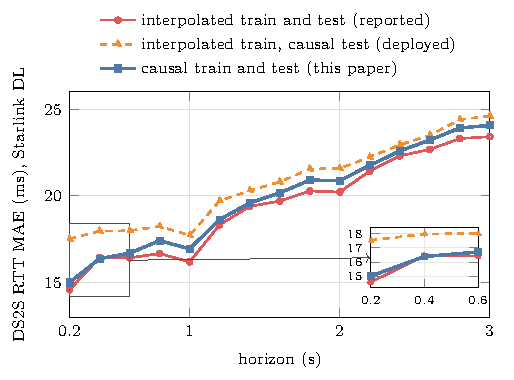
\includegraphics[width=0.85\linewidth]{figs_pdf/fr_leak.pdf}
  \caption{Effect of the interpolation leak on a trained forecaster (DS2S, Starlink DL, mean of three seeds). Trained and tested on interpolated inputs, the model reports a lower error than it reaches on the causal inputs available online. Inset: the first 0.6\,s.}
  \label{fig:leak}
\end{figure}

\paragraph{iperf alignment.} The iperf3 collector stamps each one-second report at the start of its interval, and the parsers snap it to the nearest ping row. An iperf value at row $t$ can therefore describe traffic up to about one second after $t$. The same alignment is used for every method and in the initial study. It is listed as an open problem in Section~\ref{sec:open}.
